\chapter{Risultati teorici}

\begin{teorema}\label{eulero-generica}
    Sia \(G\) un grafo planare avente \(k\) componenti connesse. Sia \(G^\varphi\) una immersione di \(G\) nel piano, allora
    \begin{equation}
        \chi(G)=V+f-\epsilon = k+1
    \end{equation}
    dove \(V\) è il numero di vertici (\(k_0\)), \(\epsilon\) il numero di archi (\(k_1\)) e \(f\) il numero di facce (\(k_2\)).
    \begin{proof}
        Procediamo per induzione sul numero di archi \( \epsilon \): \smallskip \\
        \underline{caso base \(\epsilon=0\)}, \(V=k\) vertici, \(f=1\) quindi è soddisfatta \(V-\epsilon+f = k+1\)\smallskip \\
        \underline{passo induttivo \(\epsilon \to \epsilon + 1\)}, aggiungiamo un arco al grafo
        \begin{enumerate}
            \item \textit{il nuovo arco è un loop}, in questo caso \(V \to V\), \(\epsilon \to \epsilon +1\), \(f \to f+1\), \(k \to k\) e quindi
                  \begin{equation}
                      V-(\epsilon+1)+(f+1)=V-\epsilon+f=k+1
                  \end{equation}
            \item \textit{il nuovo arco è tra due vertici appartenenti alla stessa componente connessa}, anche in questo caso \(V \to V\), \(\epsilon \to \epsilon +1\), \(f \to f+1\), \(k \to k\) e quindi
                  \begin{equation}
                      V-(\epsilon+1)+(f+1)=V-\epsilon+f=k+1
                  \end{equation}
            \item \textit{il nuovo arco connette due componenti che erano sconnesse}, in questo caso \(V \to V\), \(\epsilon \to \epsilon +1\), \(f \to f\), \(k \to k-1\) e quindi
                  \begin{equation}
                      V-(\epsilon +1)+f = (k-1) + 1 = k'+1
                  \end{equation}
                  dove \(k'=k-1\) è il numero di componenti connesse dopo l'aggiunta dell'arco.
        \end{enumerate}
    \end{proof}
\end{teorema}

\begin{corollario}[Formula di Eulero]\label{formulaeulero}
    Sia \(G\) un grafo planare connesso, allora
    \begin{equation}
        \chi(G)=V+f-\epsilon = 2
    \end{equation}
    \begin{proof}
        Direttamente dal teorema \(\ref{eulero-generica}\) con \(k=1\).
    \end{proof}
\end{corollario}

\begin{proposizione}
    Ogni suddivisione di un grafo non planare è non planare, questo implica anche che i vertici di grado 2 non influenzano la planarità del grafo.
    \begin{proof}
        Sia \(G\) grafo non planare, \(a,b\) due archi che si intersecano nell'immersione \(G^\varphi\), è evidente che suddividere \(a\) o \(b\) non andrebbe ad influire sulla non planarità del grafo.
    \end{proof}
\end{proposizione}

\begin{lemma}\label{gradifacce}
    Sia \(G\) un grafo planare, \(G^\psi\) una sua immersione nel piano, \(F_1, \dots, F_f\) le facce di \(G^\psi\) allora
    \begin{equation}
        \sum_{i=1}^f \deg(F_i) = 2\epsilon
    \end{equation}
    \begin{proof}
        Segue direttamente dal fatto che ogni arco \((u,v)\) è incedente esattamente su due facce di \(G^\psi\).
    \end{proof}
\end{lemma}

\begin{proposizione}\label{criterioNonPlan}
    Sia \(G\) planare, \(\epsilon\) il numero di archi, \(V\) il numero di vertici. Vale allora
    \begin{equation}
        \epsilon \leq 3V - 3
    \end{equation}
    Inoltre se supponiamo \(V \geq 3\) vale
    \begin{equation}
        \epsilon \leq 3V - 6
    \end{equation}
    \begin{proof}
        Sia \(V<3\). In questo caso il lemma è una diretta conseguenza della formula di Eulero (Teorema {\ref{formulaeulero}}). \\
        Sia \(V\geq 3\). \(G\) planare \(\Rightarrow\) ogni faccia ha almeno 3 lati ovvero \(\deg(F_i) \geq 3\; \forall i\). Per il lemma {\ref{gradifacce}} vale quindi
        \begin{equation}
            2\epsilon = \sum_{i=1}^f \deg(F_i) \geq \sum_{i=1}^f 3 = 3f
        \end{equation}
        Per la formula di eulero segue inoltre \(V+f-\epsilon = 2\) da cui abbiamo, moltiplicando per 3 e riarrangiando i termini
        \begin{equation}
            3\epsilon = 3V + 3f - 6
        \end{equation}
        applicando ora \(3f\leq 2 \epsilon\) otteniamo la tesi.
    \end{proof}
\end{proposizione}

\begin{lemma}\label{k5k33nonplanari}
    \(K_5\) e \(K_{3,3}\) sono grafi non planari.
    \begin{proof}
        \underline{\(K_5\)}: il grafo completo \(K_n\) ha \(\epsilon=\frac{n(n-1)}{2}\) archi. Supponendo per assurdo \(K_5\) planare dovrebbe valere la proposizione \(\ref{criterioNonPlan}\) ovvero, essendo \(V=5 \geq 3\)
        \begin{equation}
            10 = \frac{n(n-1)}{2} = \epsilon \leq 3V-6 = 9 \rightarrow \text{\Lightning}
        \end{equation}
        \underline{\(K_{3,3}\)}: Supponendo per assurdo \(K_{3,3}\) planare, sapendo \(\epsilon=3*3=9\), \(V=6\) dalla formula di eulero \(\ref{formulaeulero}\) otterremmo \(f=2-V+\epsilon=5\). \\
        Siccome \(K_{3,3}\) è bipartito, esso non contiene cicli composti da 3 archi, quindi ogni faccia ha almeno 4 lati, ovvero \(\deg(F)\geq 4 \;\forall F\) e vale \(\sum_{i=1}^{f} \deg(F_i) \geq 4*f = 20\). Applicando ora il lemma \(\ref{gradifacce}\) otteniamo l'assurdo
        \begin{equation}
            20 \leq \sum_{i=1}^{f} \deg(F_i) = 2\epsilon = 18 \rightarrow\text{\Lightning}
        \end{equation} 
    \end{proof}
    \begin{figure}[H]
        \centering
        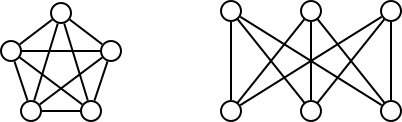
\includegraphics[scale=0.6]{img/k533.PNG}
        \caption{immersione nel piano di \(K_5\) e \(K_{3,3}\)}
    \end{figure} 
\end{lemma}


\begin{lemma}\label{lemBlocchi}
    Un grafo separabile è planare se e solo se tutti i suoi blocchi sono planari.
    \begin{proof}
        \underline{“\(\Rightarrow\)”}: banale, è evidente che se un grafo è planare allora anche i suoi sottografi lo sono.\\
        \underline{“\(\Leftarrow\)”}: notiamo che due blocchi differenti hanno al più un elemento nell'intersezione, se così non fosse i due blocchi sarebbero 2-connessi confutando l'ipotesi di massimalità. Proseguiamo ora per induzione sul numero di blocchi \(|B|\), dove \(B={\{b_i\}}_{i \in I}\) è l'insieme dei blocchi.
        \begin{itemize}
            \item \textit{caso base}: \(G\) 2-connesso quindi \(|B|=1\), \(B=\{G\}\) e la tesi equivale a “\(G \text{ planare} \Rightarrow G \text{ planare}\)”.
            \item \textit{passo induttivo}: sia \(G\) grafo composto da \(n\) cicli. Rimuoviamo da \(G\) un blocco \(b\) che si intersechi solo con un altro blocco \(b'\) nel veritce \(v\), questo deve esistere perchè altrimenti sarebbe presente un ciclo di blocchi, essi sarebbero dunque 2-connessi e di coneseguenza non massimali \(\text{\Lightning}\); 
            potrebbe anche essere che tutti i blocchi siano sconnessi e quindi la loro intersezione sarebbe sempre vuota, tuttavia questo è un caso banale in quanto è evidente che un grafo è planare se e solo se tutte le sue componenti connesse sono planari. 
            \\ Il grafo \(G'\) risultante dalla rimozione del blocco \(b\) è per ipotesi induttiva planare, disegnamo ora le immersioni nel piano di \(b\) e \(G'\) facendo in modo che il punto di intersezione \(v\) appaia in entrambe le immersioni nella faccia esterna. Possiamo ora unire tra loro le due immersioni ottenendo che \(G=G' \cup b\) è planare.
        \end{itemize}
    \end{proof}
\end{lemma}
\noindent Questo lemma ci permette di scegliere sempre un grafo 2-connesso come grafo di partenza senza perdere generalità.

\begin{lemma}
    Un grafo è planare se e solo se tutte le sue componenti conesse sono planari.
    \begin{proof}
        Caso banale dimostrato nel lemma precedente (\(\ref{lemBlocchi}\)).
    \end{proof}
\end{lemma}

%lemma usato per dimostrare il teorema sotto
\begin{lemma}\label{12.3}
    Sia \(G\) un grafo qualsiasi ottenuto splittando un vertice di \(K_5\) allora \(G\) contiene un sottografo \(TK_{3,3}\).
    \begin{proof}
        Siano \(u_1, u_2\) i due vertici risultanti dallo split di un vertice di \(K_5\). Per definizione di split ambedue i vertici hanno almeno grado 3. \(u_1\) e \(u_2\) sono adiacenti e assieme sono adiacenti a tutti i rimanenti 4 vertici. Scegliendo ora una partizione dei 4 vertici \(x,y,w,z\) t.c. \(u_1\) adiacente a \(x,y\) e \(u_2\) adiacente a \(w,z\), otteniamo un sottografo \(K_{3,3}\) con bipartizione \((u_1, w, z)\) e \((u_2,x,y)\).
    \end{proof}
\end{lemma}

%teorema usato nella dimostrazione di kuratowski
\begin{teorema}\label{minoreTK5}
    Se \(G\) ha un minore \(K_{3,3}\) allora contiene un sottografo \(TK_{3,3}\). Se \(G\) ha un minore \(K_5\) allora contiene un sottografo \(TK_{3,3}\) o \(TK_5\).
    \begin{proof}
        Supponiamo che \(G\) abbia un minore \(TK_{3,3}\) o \(TK_5\), se nel ottenere il minore non è stata coinvolta nessuna operazione di contrazione degli archi allora esso sarà anche un sottografo di \(G\). Altrimenti sia \(G_0,\dots, G_k\) sequenza di grafi ottenuta da \(G\), \(G_0\) sottografo di \(G\), l'arco \(e_i\) di \(G_{i-1}\) è contratto per ottenere \(G_i\) e \(G_k\) è \(K_{3,3}\) o \(K_5\).
        Se ogni \(e_i\) ha un endpoint di grado 2 possiamo invertire la contrazione suddividendo gli archi e trovando un sottografo \(TK_{3,3}\) o \(TK_5\). 
        \\ Altrimenti sia \(e_i\) l'arco con \(i\) massimo tra quelli con entrambi gli endpoint di grado almeno 3. Tutti gli archi contratti successivamente a \(G_i\) hanno un endpoint di grado 2, quindi \(G_i\) ha un sottografo \(TK_{3,3}\) o \(TK_5\). \(G_{i-1}\) può essere ottenuto splittando un vertice \(u \in G_i\), analizziamo ora i 3 casi:
        \begin{itemize}
            \item \textit{\(u\) appartiene a \(TK_5\)}: per il lemma \(\ref{12.3}\) \(G_{i-1}\) conterrà un sottografo \(TK_{3,3}\);
            \item \textit{\(u\) appartiene a \(TK_{3,3}\)}: anche \(G_{i-1}\) conterrà quindi \(TK_{3,3}\);
            \item \textit{\(u\) non appartiene a \(TK_{3,3}\) e \(TK_5\)}: in \(G_{i-1}\) sarà quindi ancora presente \(TK_{3,3}\) o \(TK_5\).
        \end{itemize}
    \end{proof}
\end{teorema}

\begin{teorema}[Teorema di Kuratowski]\label{Kuratowski}
    Un grafo \(G\) è planare se e solo se non contiene sottografi \(TK_{3,3}\) o \(TK_5\).
    \begin{proof}
        \underline{“\(\Rightarrow\)”}: dato il lemma \(\ref{k5k33nonplanari}\), è evidente che se un grafo \(G\) è planare non contiene sottografi omeomorfi a \(K_{3,3}\) o \(K_5\). \smallskip \\
        \underline{“\(\Leftarrow\)”}: per provare questo lato dell'implicazione dimostramo la tesi equivalente “\(G\) non planare \(\Rightarrow\) contiene \(TK_{3,3}\) o \(TK_5\)”.\\
        Consideriamo \(G\) grafo semplice, 2-connesso con \(\epsilon\) archi e procediamo per induzione su \(\epsilon\). Notiamo che se \(\epsilon \leq 6\), per il lemma \(\ref{criterioNonPlan}\) \(G\) è planare e la tesi è vera. Supponiamo quindi il teorema vero per i grafi aventi \(\epsilon-1\) archi.\\
        Consideriamo ora \(G\) non planare, \((a,b) \in E(G)\) un arco qualsiasi, \(G'=G-(a,b)\). \\
        Se \(G'\) non planare allora per ipotesi induttiva contiene \(TK_{3,3}\) o \(TK_5\), i quali saranno quindi di conseguenza contenuti anche in \(G\). \\
        Se invece \(G'\) planare, denotando con \(\kappa(a,b)\) il numero di cammini internamente disgiunti da \(a\) a \(b\) in \(G'\), siccome \(G\) è 2-connesso sappiamo \(\kappa(a,b)\geq 1\).
        \begin{enumerate}
            \item \textit{caso \(\kappa(a,b)=1\)}: questo implica che \(G'\) ha un cut vertex \(u\) in ogni cammino da \(a\) a \(b\). Aggiungiamo gli archi \((a,u)\) e \(b,u\) a \(G'\) se non sono già presenti e otteniamo un grafo \(H\). Denotiamo \(Ha,\; Hb\) i blocchi di \(H\) contenenti \(a\) e \(b\).
            \\ Dimostriamo ora che \(Ha\) o \(Hb\) è non planare, se entrambi fossero planari infatti potremmo disegnare le loro immersioni nel piano lasciando gli archi \((a,u)\), \((b,u)\) nella faccia esterna, “incollarli” tra loro al vertice \(u\) rimuovere  \((a,u)\), \((b,u)\) e ottenere così un immersione planare di \(G\). Questo è un assurdo essendo \(G\) non planare.\\
            Supponiamo quindi \(Ha\) non planare, per ipotesi induttiva contiene come sottografo \(TK_{3,3}\) o \(TK_5\). Tale sottografo essendo \(G'\) planare conterrà l'arco \((a,u)\), rimpiazziando quindi \((a,u)\) con il cammino formato dall'arco \((a,b)\) e dal cammino \(b \to u\) in \(Hb\), il risultato sarà un sottografo \(TK_{3,3}\) o \(TK_5\) in \(G\).
            \item \textit{caso \(\kappa(a,b)=2\)}: siano \(P1\), \(P2\) due cammini internamente disgiunti da \(a\) a \(b\) in \(G'\). Siccome \(\kappa(a,b)=2\) \(\exists v \in P1, u \in P2\) t.c.\@ tutti i cammini da \(a \to b\) contengono uno tra
            \(\{ u,v \} \) e \(G'-\{ u,v \} \) è disconnesso. Siano ora \(Ka\), \(Kb\) le due componenti connesse di \(G'-\{ u,v\} \) 
            contenenti rispettivamente \(a\) e \(b\). Denotiamo inoltre \(G_a' \doteq Ka \cup \{ u,v \},\; G_b' \doteq Kb \cup \{ u,v\} \).
            \\ Aggiungiamo ora un vertice \(x\) a \(G_a'\) adiacente a \(u,v,a\) e similmente un vertice \(y\) a \(G_b'\) adiacente a \(u,v,b\), denotiamo questi grafi \(Ha,\; Hb\). 
            \\ Proviamo ora per assurdo almeno uno tra \(Ha\) e \(Hb\) è non planare. Siccome il vertice \(x\) ha grado 3 in \(Ha\), ci sono 3 facce incidenti su esso. Disegnamo un immersione planare di \(Ha\) facendo in modo che le facce contenenti gli archi \((u,x), (v,x)\) siano le facce esterne. Similmente disegnamo \(Hb\) in modo che \((u,y),(v,y)\) siano nella faccia esterna. Ora “incolliamo” \(Ha\) e \(Hb\) nei vertici \(u\) e \(v\), cancelliamo \(x\) e \(y\) e aggiungendo l'arco \((a,b)\)
            otterremmo una immersione planare di \(G\) \(\rightarrow \text{\Lightning}\). Concludiamo quindi che uno tra \(Ha\) e \(Hb\) è non planare.\\
            Supponendo \(Ha\) non planare allora per ipotesi induttiva contiene un sottografo \(TK_{3,3}\) o \(TK_5\). Se tale sottografo non contiene \(x\) allora è contenuto anche in \(G\) e la dimostrazione è conclusa. Supponiamo quindi che il sottografo contenga \(x\), in questo caso \(Hb\) sarà 2-connesso, in quanto \(G\) lo è. \(Hb\) conterrebbe quindi due cammini internamente disgiunti \(b \to u,\; b\to v\). 
            Questi due cammini assieme all'arco \((a,b)\) possono essere utilizzati per rimpiazzare gli archi \((u,x),(v,x),(a,x)\) di \(Ha\) ottenendo così un sottografo \(TK_{3,3}\) o \(TK_5\) in \(G\).
            \item \textit{caso \(\kappa(a,b)\geq 3\)}: siano \(P1\), \(P2\), \(P3\) due cammini internamente disgiunti da \(a\) a \(b\) in \(G'\). Consideriamo una immersione nel piano di \(G'\), ogni coppia di cammini \(P1 \cup P2, P1 \cup P3, P2 \cup P3\) crea un ciclo la cui immersione nel piano sarà una curva di Jordan. Uno dei tre cammini sarà quindi contenuto nella curva di Jordan formata dagli altri, supponiamo \(P2\) contenuto all'interno di \(P1 \cup P3\).
            L'arco \((a,b)\) può essere immerso all'interno di \(P1 \cup P2\), all'interno di \(P2 \cup P3\) o all'esterno di \(P1 \cup P3\). Siccome \(G\) è non planare ognuna di queste tre regioni \(Pi\) deve contenere un cammino da un vertice interno a \(Pi\) a uno interno a \(Pj\). Sia \(P12\) un cammino da \(u_1 \in P1\) a \(u_2 \in P2\), \(P13\) da \(v_1 \in P1\) a \(u_3 \in P3\), \(P13\) da \(u_2 \in P2\) a \(v_3 \in P3\).\\
            \(\forall i\) se \(u_i \neq v_i\) contraiamo l'arco tra essi, aggiungendo ora l'arco \((a,b)\) il grafo risultante sarà un minore \(TK_5\) di \(G\). Quindi per il teorema \(\ref{minoreTK5}\) \(G\) conterrà un sottografo \(TK_5\) o \(TK_{3,3}\).
            \begin{figure}[H]
                \centering
                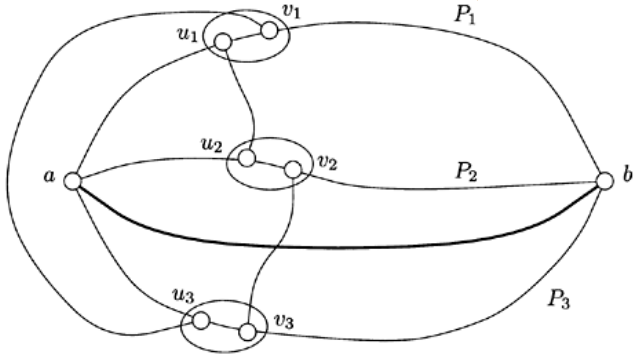
\includegraphics[scale=0.6]{img/minoreTK5.PNG}
                \caption{minore \(TK_5\) di \(G\)}
            \end{figure}
        \end{enumerate}
    \end{proof}
\end{teorema}
\noindent Si può riformulare il teorema precedente in termine di minori.
\begin{teorema}[Teorema di Wagner]
    Un grafo \(G\) è planare se e solo se non ha \(K_{3,3}\) o \(K_5\) come minori.
    \begin{proof}
        \underline{“\(\Rightarrow\)”}: se \(G\) planare ovviamente non ha come minori \(K_{3,3}\) o \(K_5\). \\
        \underline{“\(\Leftarrow\)”}: se \(G\) non ha \(K_{3,3}\) o \(K_5\) come minori allora non ha nemmeno sottografi \(TK_{3,3}\) o \(TK_5\) e quindi è planare per il teorema di Kuratowski \(\ref{Kuratowski}\).
    \end{proof}
\end{teorema}
